\unitheader{A}{Learning-rate scaling with AdamW}{}

Optimal learning rates depend on other hyperparameters, such as batch size.
How should they change as we scale up the data or model?

We might imagine that there are many possible answers to this question. Since the model is the same, and the optimal learning rate is often fairly stable, we might imagine the optimal learning rate stays similar. Or, we might look at the theory of convex optimization and conclude that, based on the convergence theorems that the right thing to do would be to decrease learning rates at rates of $O(1/\sqrt{T})$ or $O(1/T)$ for $T$ steps.

This is a simple, but surprisingly complex and consequential topic. Even large scale, serious empirical efforts on this question leads to disagreement, as you can see in this example taken from the StepFun learning rate scaling paper.

\begin{center}
  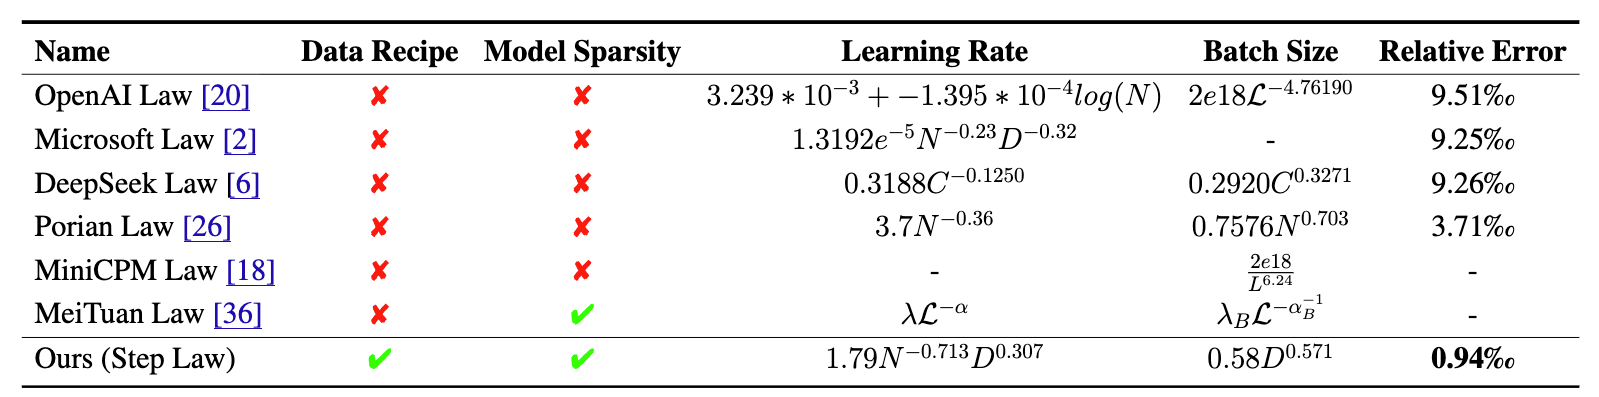
\includegraphics[width=0.78\linewidth]{figures/stepfun}\\
  {\footnotesize\itshape Examples of various \emph{scaling rules} for hyperparameters identified across the literature. Note the broad disagreement between credible papers and organizations.}
\end{center}

We will now study how learning rate scaling works in our $d8$ system and see if we can build intuition for what types of scaling rules are plausible. Throughout, let $D$ denote the training-token budget.

\needspace{16\baselineskip}
\begin{problem}{When can training on less data guide large scale runs? (9 new runs)}
Use the baseline model and default training settings above. Vary LR and the
training-token budget, keeping the other settings fixed.
For parts (a) and (b), analyze the \providedSweeps{} or the starter's CSV.
Fit the curves and make the plots yourself.

\begin{parts}
\item \textbf{Learn from small training budgets (provided runs).}
At 153.6M, 307.2M, and 614.4M tokens, investigate how final validation loss
changes with peak LR using the provided measurements at $\{.0015,.003,.006\}$. For each scale, fit a curve mapping peak LR to loss, and use this to estimate
the optimal LR. Use these optima to propose a scaling rule in the training-token budget.
Plot the fitted optima and your rule. What trend do you observe?

\needspace{4\baselineskip}
\item \textbf{Predict before increasing the budget (provided runs).}
Record your predicted optimal LRs at 1.2288B, 1.8432B, and 2.4576B tokens
before inspecting the provided measurements at these budgets.
Then fit their loss--LR curves and compare your predictions with the fitted optima. Does the trend from the small budgets continue?

\item \textbf{Compare and test two scaling rules (5 new runs).}
Fit one learning-rate power law over all six source budgets from parts (a) and (b),
and another over only 1.2288B, 1.8432B, and 2.4576B tokens.
Use each to predict the optimal LR at 4.9152B. Which prediction do you expect
to give the lower loss, and why?

Train at both predicted LRs and at target-grid LRs $\{.0015,.003,.006\}$.
Compare your predictions with the fitted target optimum and report their measured
loss gaps relative to the best sampled LR in the target grid. Did you find gains from using the smaller model fits? Think about bias-variance tradeoffs in fitting scaling laws, and how far you can extrapolate your scaling law fits.

\needspace{19\baselineskip}
\item \textbf{Hyperball versus AdamW (recommended: 4 new runs).}
The shape and predictability of learning rate scaling might vary significantly across optimizers, and one of the motivations for new and exotic optimization methods is that they may scale more predictably than the standard ones.

To this end we will explore Hyperball, which is a simple modification of the well-studied Adam optimizer. Hyperball uses an Adam direction but constrains each selected weight matrix to
keep its initial norm. For a linear-layer weight matrix $W_t$, let $U_{t}$ be Adam update direction. Write
$\lVert\cdot\rVert_F$ for the Frobenius norm (the square root of the sum of
squared entries). For nonzero norms, the Hyperball update is
\[
  W_{t+1}
=\frac{\lVert W_t\rVert_F}{\lVert\widetilde W_{t+1}\rVert_F}
\widetilde W_{t+1}
\qquad
\widetilde W_{t+1}
= W_t-\eta_t\frac{\lVert W_t\rVert_F}{\lVert U_t\rVert_F}U_t.
\]
We propose an update $\widetilde W_{{t+1}}$ by scaling the standard Adam update relative to the weight norm, and enforce that the norm remains the same after the step. Since hyperball already controls the norms, Hyperball uses no weight decay. Embeddings, normalization parameters, and biases use ordinary Adam.
The supplied runs use peak LR $(.000656/.00630)\eta\approx .1041\eta$ for
these Adam parameters, where $\eta$ is the listed Hyperball peak LR.
Apply the same warmup and decay multiplier to both groups, and keep this LR
ratio fixed in your target runs.

Use the 24 supplied Hyperball runs (\texttt{P1d}) at 153.6M, 307.2M,
and 614.4M tokens, with eight LRs at each budget. Fit an optimum at each
of these three budgets and fit a power law to those optima. Compare its trend
with AdamW fitted to the same three budgets; no larger Hyperball source budgets
are supplied. Record a prediction at 1.2288B tokens before running that target.
Test the predicted LR and three nearby LRs of your choice (up to four new runs,
reusing duplicates). Compare the prediction with the best sampled target loss.
Does the optimal LR vary more regularly with budget? Discuss the uncertainty
of extrapolating from only three source budgets.

\item \textbf{Explore schedule variants (optional).}
Thus far, we have studied optimal LR scaling for a single schedule. Do our findings transfer across learning rate schedules? Can we \emph{directly} transfer the optimal LR from one schedule to another?
Explore different learning-rate schedules, such as cosine decay or a constant
learning rate, using the same methodology.
\end{parts}
\end{problem}
\clearpage
